%%%%%%%%%%%%%%%%%%%%%%%%%%%%%%%%%%%%%%%%%%%%%%%%%%%%%%
% MDLN — Leveraging AI and Synthetic Data in TAF-based Research
% Becky Staiger, UC Berkeley
% September 15, 2026
%%%%%%%%%%%%%%%%%%%%%%%%%%%%%%%%%%%%%%%%%%%%%%%%%%%%%%
\documentclass[notes,11pt, aspectratio=169, xcolor={table}]{beamer}

\usepackage{helvet}
\usepackage[default]{lato}
\usepackage{array}

% Appendix numbers not counted
\setbeamertemplate{navigation symbols}{}
\newcommand{\backupbegin}{
   \newcounter{framenumberappendix}
   \setcounter{framenumberappendix}{\value{framenumber}}
}
\newcommand{\backupend}{
   \addtocounter{framenumberappendix}{-\value{framenumber}}
  \addtocounter{framenumber}{\value{framenumberappendix}}
}

\usepackage{tikz}
\usepackage{verbatim}
\setbeamertemplate{note page}{\pagecolor{yellow!5}\insertnote}
\usetikzlibrary{positioning}
\usetikzlibrary{calc}
\usetikzlibrary{arrows}
\usetikzlibrary{arrows.meta}
\usetikzlibrary{decorations.markings}
\usetikzlibrary{shapes.misc}
\usetikzlibrary{matrix,shapes,arrows,fit,tikzmark}
\usepackage{amsmath}
\usepackage{mathpazo}
\usepackage{hyperref}
\usepackage{graphicx}
\usepackage{multirow}
\usepackage{dcolumn}
\usepackage{bbm}
\usepackage{adjustbox}
\newcolumntype{d}[0]{D{.}{.}{5}}
\newcolumntype{L}[1]{>{\raggedright\arraybackslash}p{#1}}
\usepackage{mathtools}
\setcounter{footnote}{1}
\usepackage{soul}
\usepackage[flushleft]{threeparttable}

\usepackage[space]{grffile}
\usepackage{booktabs}
\newcommand{\tabitem}{~~\llap{\textbullet}~~}

% COLORS (TOL Color Palette)
\definecolor{blue}{RGB}{51, 34, 136}
\definecolor{red}{RGB}{204, 102, 119}
\definecolor{yellow}{RGB}{221, 204, 119}
\definecolor{green}{RGB}{68, 170, 153}
\definecolor{lblue}{RGB}{136, 204, 238}

\hypersetup{
  colorlinks=false,
  linkbordercolor = {white},
  linkcolor = {blue}
}

%% Beige off-white background
\definecolor{MyBackground}{RGB}{248, 248, 253}
\setbeamercolor{background canvas}{bg=MyBackground}

\newenvironment{transitionframe}{
  \setbeamercolor{background canvas}{bg=lblue}
  \begin{frame}}{
    \end{frame}
}

\setbeamercolor{frametitle}{fg=blue}
\setbeamercolor{title}{fg=blue}
\setbeamertemplate{footline}[frame number]
\setbeamertemplate{navigation symbols}{}
\setbeamertemplate{itemize items}{-}
\setbeamercolor{itemize item}{fg=black}
\setbeamercolor{itemize subitem}{fg=black}
\setbeamercolor{enumerate item}{fg=black}
\setbeamercolor{enumerate subitem}{fg=black}
\setbeamercolor{button}{bg=blue,fg=white,}

\setbeamercolor{section in toc}{fg=black}
\setbeamercolor{subsection in toc}{fg=black}
\setbeamersize{text margin left=1em,text margin right=1em}

\newenvironment{wideitemize}{\itemize\addtolength{\itemsep}{3pt}}{\enditemize}

\usepackage{appendixnumberbeamer}

%%% Deck-specific helpers %%%
\usepackage{inconsolata}
\newcommand{\code}[1]{{\ttfamily\small #1}}
\newcommand{\keyline}[1]{\vspace{0.4em}{\color{blue}\textbf{#1}}}

%%%%%%%%%% Title  %%%%%%%%%%
\title{Leveraging AI and Synthetic Data in TAF-based Research}
\author[shortname]{Becky Staiger\\
\normalsize{University of California, Berkeley\\}}
\date{Medicaid Data Learning Network \\ September 15, 2026}
%%%%%%%%%%%%%%%%%%%%%%%%

\begin{document}

\begin{frame}[plain]
\maketitle
\end{frame}

%=========================================================
\begin{frame}{Overview}

\begin{wideitemize}
\item What we want to do: use Medicaid (and Medicare) administrative claims for research
\item Problem: this is often hard to do
\begin{wideitemize}
\item Expensive!
\item Getting access takes a long time
\item Secure servers with data may be ``clunky,'' often don't have internet
\end{wideitemize}
\item Goal: become more \underline{efficient} --- higher quality work in a reasonable amount of time
\end{wideitemize}
\end{frame}

\begin{frame}{The proposal: synthetic data}

\vspace{0.6em}

Build \textbf{\color{blue}synthetic data} to train the code on

\begin{wideitemize}
\item Mirror the real files --- structure, naming, defects, moments
\item Write and test the whole pipeline locally, with full tooling
\item Transfer in code that already works
\end{wideitemize}

\vspace{0.6em}

Today: a \textbf{\color{blue}blueprint} for generating synthetic MAX + TAF data
\begin{wideitemize}
\item GitHub repo: \url{https://github.com/beckystaiger87/synthetic-mcaid-claims-blueprint}
\item You generate your own synthetic data, for your states, years, files and question.
\item Why not make synthetic data available?
\begin{wideitemize}
\item What I need in my project may not be relevant to you (and vice versa)
\item To be useful, would take up too much space
\end{wideitemize}
\end{wideitemize}
\vspace{0.6em}
Note: this talk is built around access via VRDC, but is equally relevant for physical-file access
\end{frame}

%=========================================================
\begin{transitionframe}
\begin{center}{\Large\color{blue}\textbf{How the synthetic data is built}}\end{center}
\end{transitionframe}

%=========================================================
\begin{frame}{The shape of it}
\vspace{-0.2em}
\begin{center}
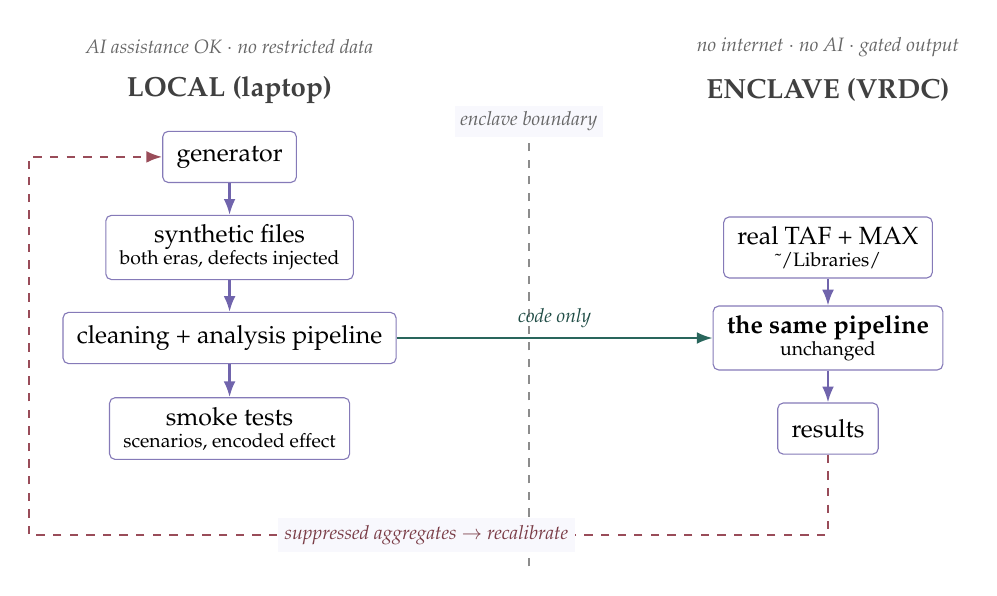
\begin{tikzpicture}[
  font=\small,
  box/.style={draw=blue!60, fill=white, rounded corners=2pt, minimum height=6.5mm,
              inner xsep=5pt, align=center},
  lab/.style={font=\scriptsize\itshape, text=black!60},
  ar/.style={-{Latex[length=2mm]}, draw=blue!70, thick}
]
\node[font=\normalsize\bfseries, text=black!75] at (0,3.15)   {LOCAL (laptop)};
\node[font=\normalsize\bfseries, text=black!75] at (7.6,3.15) {ENCLAVE (VRDC)};
\node[lab] at (0,3.7)   {AI assistance OK $\cdot$ no restricted data};
\node[lab] at (7.6,3.7) {no internet $\cdot$ no AI $\cdot$ gated output};

\node[box] (gen)   at (0,2.3)  {generator};
\node[box] (synth) at (0,1.15) {synthetic files\\[-3pt]\scriptsize both eras, defects injected};
\node[box] (pipe)  at (0,0)    {cleaning + analysis pipeline};
\node[box] (val)   at (0,-1.15){smoke tests\\[-3pt]\scriptsize scenarios, encoded effect};
\draw[ar] (gen)--(synth); \draw[ar] (synth)--(pipe); \draw[ar] (pipe)--(val);

\node[box] (real)  at (7.6,1.15) {real TAF + MAX\\[-3pt]\scriptsize \textasciitilde/Libraries/};
\node[box] (pipe2) at (7.6,0)    {\textbf{the same pipeline}\\[-3pt]\scriptsize unchanged};
\node[box] (res)   at (7.6,-1.15){results};
\draw[ar] (real)--(pipe2); \draw[ar] (pipe2)--(res);

\draw[dashed, thick, black!45] (3.8,-2.9) -- (3.8,2.75);
\node[lab, fill=MyBackground, inner sep=2pt] at (3.8,2.75) {enclave boundary};
\draw[ar, green!60!black] (pipe.east) -- node[lab, above, text=green!45!black]{code only} (pipe2.west);
\draw[-{Latex[length=2mm]}, red!75!black, dashed, thick]
   (res.south) -- (7.6,-2.5) -- (-2.55,-2.5) -- (-2.55,2.3) -- (gen.west);
\node[lab, text=red!60!black, fill=MyBackground, inner sep=2.5pt] at (2.5,-2.5)
   {suppressed aggregates $\rightarrow$ recalibrate};
\end{tikzpicture}
\end{center}
\vspace{-0.3em}
\keyline{One direction carries code. The other carries only suppressed aggregates.}
\end{frame}

%=========================================================
\begin{frame}{Six ingredients}

\vspace{0.3em}
\footnotesize
\begin{center}
\begin{tabular}{c L{0.30\textwidth} L{0.50\textwidth}}
\toprule
 & \textbf{Ingredient} & \textbf{What it contributes} \\
\midrule
\textbf{1} & Variable names from public data dictionaries
           & the synthetic columns \emph{are} the real columns; a check flags any that drift \\[4pt]
\textbf{2} & Mirror the file structure
           & header/line splits, 12 monthly columns, slot$\times$month grids, two person ids \\[4pt]
\textbf{3} & Harmonize eras
           & one pipeline reads \textbf{both MAX and TAF} \\[4pt]
\textbf{4} & Inject known data-quality issues
           & the cleaner has something to catch --- clean data tests nothing \\[4pt]
\textbf{5} & Calibrate to real moments
           & public sources first, then suppression-compliant CMS aggregates \\[4pt]
\textbf{6} & Encode truths about the DGP
           & and test that your analysis code recovers them \\
\bottomrule
\end{tabular}
\end{center}

\vspace{0.6em}
\normalsize
\begin{center}\small
On \textbf{1}: dictionaries are public, but naming differs by vintage and by provider.
The check flags a mismatch; \textbf{you fix it by hand against the files you actually have}.
\end{center}

\vspace{0.4em}
\keyline{More details on 4, 5 and 6.}
\end{frame}

%=========================================================
\begin{frame}[fragile]{4 --- inject the defects}

\vspace{-0.3em}
\footnotesize
\begin{center}
\begin{tabular}{L{0.235\textwidth} L{0.245\textwidth} L{0.09\textwidth} L{0.30\textwidth}}
\toprule
\textbf{Defect} & \textbf{Cause} & \textbf{Rate} & \textbf{Caught by} \\
\midrule
Missing servicing NPI & LPI sent instead & 5--25\% & xwalk, then drop blanks \\[3pt]
Off-year service dates & late-filed claims & \textasciitilde1\%\,$\uparrow$ & year from the date column \\[3pt]
Exact duplicate rows & resubmissions & \textasciitilde1\%\,$\uparrow$ & \code{unique()} on natural key \\[3pt]
Duplicate bene-years on PS/DE & cross-state movers; enrollment corrections & \textasciitilde0.5\% & drop all rows for that bene-year \\[3pt]
Unlinked BENE\_ID & CCW linkage failed & 1--5\% & fallback key \\[3pt]
BENE\_ID reassigned & MAX\,$\rightarrow$\,TAF & \textasciitilde5\% & era crosswalk \\[3pt]
Mixed NDC length & 11 vs 13 char & \textasciitilde10\% & normalize on read \\[3pt]
Constant sentinel & one plan's placeholder & 1 plan & tabulate \textbf{by submitter} \\
\bottomrule
\end{tabular}
\end{center}

\vspace{0.5em}
\normalsize
$\uparrow$ = injected \emph{above} the real rate, so a small sample still shows it. Record that
next to the parameter:

\vspace{0.2em}
\begin{semiverbatim}\small
  offyear_date_rate = 0.015,  \color{blue}# ABOVE REAL (~0.3%) for detectability
\end{semiverbatim}

\vspace{0.1em}
{\small Without the comment, someone later ``corrects'' it to the true rate and switches the
test off.}
\end{frame}

%=========================================================
\begin{frame}{5 --- calibrate to real moments: public data}

\vspace{0.4em}
\begin{center}
\begin{tabular}{L{0.32\textwidth} L{0.56\textwidth}}
\toprule
\textbf{Public source} & \textbf{Calibrates} \\
\midrule
MBES / CMS-64 & enrollment by state-year \\[3pt]
DQ Atlas & injection rates; which state-years are unusable \\[3pt]
KFF state summaries & eligibility-group mix \\[3pt]
NPPES & a real provider universe \\
\bottomrule
\end{tabular}
\end{center}

\vspace{1.1em}
\keyline{All publicly available, unrestricted information.}

\vspace{0.7em}
\small
Note: the NPPES is useful in generating synthetic data with real NPI's. This can be used to reproduce a match rate you'd actually face in the data, should you match on other NPI-identified datasets.
\end{frame}

%=========================================================
\begin{frame}{5 --- calibrate to real moments: server data}
\vspace{-0.4em}
\begin{center}
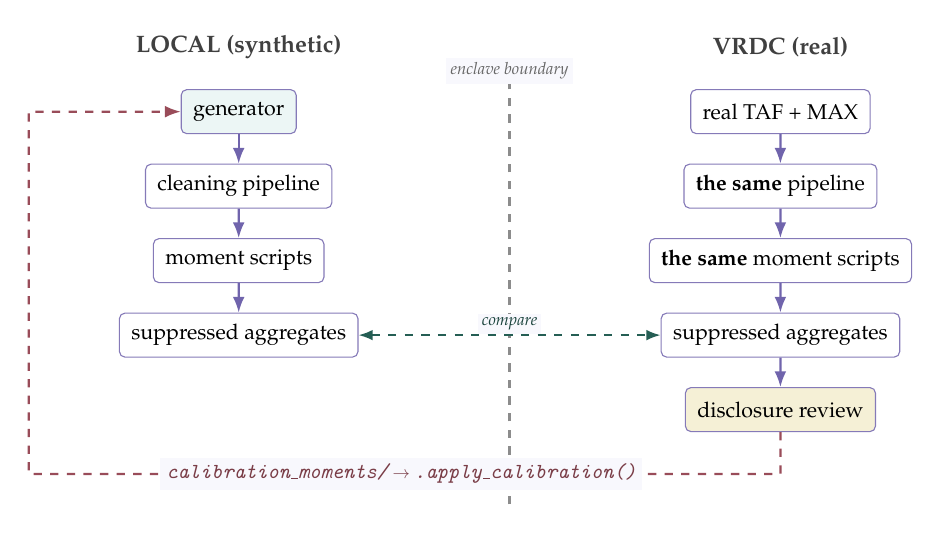
\begin{tikzpicture}[
  scale=0.86, every node/.style={transform shape},
  font=\small,
  box/.style={draw=blue!60, fill=white, rounded corners=2pt, minimum height=6.5mm,
              inner xsep=5pt, align=center},
  lab/.style={font=\scriptsize\itshape, text=black!60},
  ar/.style={-{Latex[length=2mm]}, draw=blue!70, thick}
]
\node[font=\normalsize\bfseries, text=black!75] at (0,3.15) {LOCAL (synthetic)};
\node[font=\normalsize\bfseries, text=black!75] at (8,3.15) {VRDC (real)};
\node[box, fill=green!10] (gen) at (0,2.2)  {generator};
\node[box] (p1) at (0,1.1)  {cleaning pipeline};
\node[box] (m1) at (0,0)    {moment scripts};
\node[box] (d1) at (0,-1.1) {suppressed aggregates};
\draw[ar] (gen)--(p1); \draw[ar] (p1)--(m1); \draw[ar] (m1)--(d1);
\node[box] (r2) at (8,2.2)  {real TAF + MAX};
\node[box] (p2) at (8,1.1)  {\textbf{the same} pipeline};
\node[box] (m2) at (8,0)    {\textbf{the same} moment scripts};
\node[box] (d2) at (8,-1.1) {suppressed aggregates};
\node[box, fill=yellow!30] (rev) at (8,-2.2) {disclosure review};
\draw[ar] (r2)--(p2); \draw[ar] (p2)--(m2); \draw[ar] (m2)--(d2); \draw[ar] (d2)--(rev);
\draw[dashed, thick, black!45] (4,-3.6) -- (4,2.8);
\node[lab, fill=MyBackground, inner sep=2pt] at (4,2.8) {enclave boundary};
\draw[{Latex[length=1.8mm]}-{Latex[length=1.8mm]}, green!55!black, thick, dashed]
  (d1.east) -- node[lab, above, text=green!40!black, fill=MyBackground, inner sep=1.5pt]
  {compare} (d2.west);
\draw[-{Latex[length=2mm]}, red!75!black, dashed, thick]
  (rev.south) -- (8,-3.15) -- (-3.1,-3.15) -- (-3.1,2.2) -- (gen.west);
\node[lab, text=red!60!black, fill=MyBackground, inner sep=2.5pt] at (2.4,-3.15)
  {\code{calibration\_moments/} $\rightarrow$ \code{.apply\_calibration()}};
\end{tikzpicture}
\end{center}

\end{frame}

%=========================================================
\begin{frame}{6 --- encode truths about the data-generating process}

\begin{wideitemize}
\item Set a \textbf{``known'' effect} in the generator --- e.g. losing your usual provider
      reduces the probability of an E\&M visit in a given month by \textbf{15 percentage
      points} (0.36 $\rightarrow$ 0.21)
\item Say what unit it lives at: here, an \textbf{enrolled bene-month}
\item Write it to a \textbf{truth file}. {\color{red}Analysis code never reads it}
\item Run your estimator. Make sure you can recover this estimate.
\end{wideitemize}

\vspace{1.2em}
\begin{center}
\begin{minipage}{0.88\textwidth}
\footnotesize The setting is from Staiger (2022), \emph{Disruptions to the Patient-Provider
Relationship and Patient Utilization and Outcomes}, J.\ Health Econ.\ 81:102574. The estimated effect in the paper is $-$3.7pp on a 0.679 pre-exit base, per bene-quarter; the magnitude encoded
here is larger for sake of illustration.
\end{minipage}
\end{center}

\end{frame}

%=========================================================
\begin{frame}[fragile]{One estimator, two denominators}

\small
\begin{semiverbatim}
\$ Rscript example/run_all.R

  [bene-month] estimate: \color{green}-0.1425\color{black} (SE 0.0050) CI [-0.1523, -0.1327]
  encoded:  -0.1500
  \color{green}PASS\color{black} - CI covers the encoded effect.

  [claims-file months] estimate: \color{red}-0.1667\color{black} (SE 0.0076) CI [-0.1817, -0.1518]
  encoded:  -0.1500
  rows: 91,998 of 207,694 enrolled bene-months (\color{red}56% of the panel is gone\color{black})
  \color{red}FAIL\color{black} - off by 11%.
\end{semiverbatim}

\vspace{0.7em}
\normalsize
\begin{wideitemize}
\item The effect is a probability \textbf{per enrolled bene-month} --- so months with
      \textbf{no claim} belong in the denominator
\item Build the panel from the \textbf{claims} file and those months are simply absent
\item Both run without error $\cdot$ both significant $\cdot$ both correctly signed
\end{wideitemize}

\vspace{0.5em}
\keyline{Losing your provider shrinks the outcome \emph{and} the sample.}
\end{frame}


%=========================================================
\begin{transitionframe}
\begin{center}{\Large\color{blue}\textbf{Workflow, and where AI fits}}\end{center}
\end{transitionframe}

%=========================================================
\begin{frame}{Thought partner, not autonomous agent}

\vspace{0.4em}
\begin{wideitemize}
\item \textbf{Start from a puzzle, not a coding request.}\\
  \small ``I'm seeing Y --- what could explain it?'' produces understanding. ``Write me a
  query that does X'' produces code that may answer the wrong question.
\item \textbf{The agent has amnesia.}\\
  \small Every session starts ignorant. The markdown files \emph{are} the institutional
  memory --- documentation is an output, not an afterthought.
\item \textbf{Verification through redundancy.}\\
  \small Two implementations agreeing is evidence. One running without error is none.
\item \textbf{Adversarial review requires separation.}\\
  \small The instance that wrote the code cannot audit it.
\item \textbf{Legible or unchecked.}\\
  \small A skimmed result is an unverified result --- so how a finding is written is part of
  whether it gets verified at all.
\end{wideitemize}


\vspace{0.4em}
\begin{center}\small
Harness: Scott Cunningham's \code{mixtapetools}, adapted for enclave constraints
\end{center}
\end{frame}



%=========================================================
\begin{frame}[fragile]{Check it as you build it}

Every construction step writes a \textbf{QC report} next to its output. Committed, not scratch.

\vspace{0.5em}
\footnotesize
\begin{semiverbatim}
\color{blue}# QC — 02_pull_ot                      0.5s  ·  FLAG (1)\color{black}

  OK     de-dup removes under 5% of lines            1.0%
  OK     crosswalk resolved some legacy ids          13,138 resolved
  OK     under 15% dropped, unresolvable servicing   7.5%
  OK     MAX carries no billing NPI
  \color{red}FLAG   no plan reports a single billing NPI     CA0000002\color{black}
\end{semiverbatim}

\vspace{0.8em}
\normalsize
\begin{wideitemize}
\item \textbf{Catches a nonsensical number now}, while you still remember what you changed
\item \textbf{Records the intermediate.} Six weeks on, ``when did this change?'' has an answer
\end{wideitemize}

\end{frame}


%=========================================================
\begin{frame}{Three checks}

\vspace{-0.2em}
\scriptsize
\begin{center}
\begin{tabular}{L{0.09\textwidth} L{0.22\textwidth} L{0.26\textwidth} L{0.28\textwidth}}
\toprule
 & \textbf{QC per step} & \textbf{Blindspot} & \textbf{Referee 2} \\
\midrule
Asks & does this number make sense? & can you see what's in front of you? & is this implemented correctly? \\[3pt]
When & as you write the step & output appears, \emph{before} interpreting & end of an arc \\[3pt]
Session & inline & same --- proximity is the point & \textbf{fresh} --- independence is the point \\[3pt]
Catches & rows lost without a reason & the unexplained spike, the check nobody ran & join fan-out, clustering, disclosure \\[3pt]
Cost & seconds & minutes & hours \\
\bottomrule
\end{tabular}
\end{center}

\vspace{0.6em}
\begin{center}
\begin{tabular}{L{0.42\textwidth} c c c}
\toprule
 & \textbf{QC} & \textbf{Blindspot} & \textbf{Referee 2} \\
\midrule
A diagnostic you will cite anywhere & \textbf{run} & \textbf{run} & --- \\
A step other steps depend on & \textbf{run} & \textbf{run} & at arc end \\
Anything feeding a headline number & \textbf{run} & \textbf{run} & \textbf{run} \\
\bottomrule
\end{tabular}
\end{center}

\vspace{0.7em}
\small
\begin{center}
\begin{minipage}{0.92\textwidth}
{\color{red}\textbf{Do not follow the last two blindly.}} A generated list of concerns is a list
of \emph{candidates}, and not all are worthwhile to implement. 
\end{minipage}
\end{center}
\end{frame}

%=========================================================
%=========================================================
\begin{frame}{Working example}

\vspace{0.2em}
\small
Project question: how does physician practice ownership determine a physician's Medicaid participation?  MAX/TAF 2012 -- 2022, three specialties, event studies leveraging acquisition dates

\begin{wideitemize}
\item Team members: 4 --- 2 of us working with the data, 1 VRDC seat
\item Create synthetic data
\item Train code on the synthetic data (SAS, R)
\item Export NPI-level, suppression-compliant measures of provider participation; link to our existing ownership database (from this \href{https://academic.oup.com/healthaffairsscholar/article/4/7/qxag178/8729615?login=false&utm_source=authortollfreelink&utm_campaign=healthaffairsscholar&utm_medium=email}{\textcolor{blue}{paper}})
\item Conduct analyses outside of server to troubleshoot (get 99\% of the way there)
\item At the end: run in the VRDC
\end{wideitemize}

\end{frame}




%=========================================================
\begin{frame}{Limitations}

\vspace{0.8em}
\begin{wideitemize}
\item \textbf{Most real bugs are invisible here.} A filter, not a proof
\item \textbf{Only the defects you already know about.} Real data still surprises you
\item \textbf{The numbers mean nothing.} A test harness, not data
\item \textbf{Validates code, not design.} Parallel trends hold because you built them in
\item \textbf{It rots.} A stale generator breaks pipeline code in confusing ways
\item \textbf{Calibration needs server access.} You cannot do it before you are in
\end{wideitemize}

\vspace{1.2em}
\keyline{It buys the cheap bugs, so server time goes to the expensive ones.}
\end{frame}


\begin{transitionframe}
\begin{center}{\Large\color{blue}\textbf{Take-aways}}\end{center}
\end{transitionframe}

%=========================================================
\begin{frame}{Who might use this}

\vspace{0.6em}
\begin{wideitemize}
\item[] \keyline{A research team --- especially when only one member has a VRDC seat}
\begin{itemize}\small
\item everyone else writes and tests against synthetic files
\item the seat-holder runs finished code instead of debugging it
\item no waiting for a second seat to be approved and paid for
\end{itemize}

\vspace{1.0em}
\item[] \keyline{Students}
\begin{itemize}\small
\item learn what a TAF pipeline looks like with no DUA
\item a real task with a checkable answer: recover the encoded effect
\item productive during the 6--18 months access takes
\end{itemize}
\end{wideitemize}

\vspace{1.2em}
\begin{center}
\begin{minipage}{0.86\textwidth}
\color{blue}\textbf{And anyone who wants their pipeline checked.}\\[4pt]
\normalsize\color{black} Nobody can rerun a TAF analysis without a DUA --- so nobody does.
Anyone can run the generator plus the pipeline.
\end{minipage}
\end{center}
\end{frame}

%=========================================================
\begin{frame}{Resources}

\vspace{0.8em}
\begin{center}
{\large These slides and the synthetic-data blueprint}\\[5pt]
\code{github.com/beckystaiger87/synthetic-mcaid-claims-blueprint}
\end{center}

\vspace{0.8em}
\footnotesize
\begin{center}
\begin{tabular}{L{0.20\textwidth} L{0.66\textwidth}}
\toprule
\code{SYNTHETIC-} & the specification: six ingredients, reader contract, \\
\code{DATA-BLUEPRINT.md} & \hspace{0pt}build order \\[3pt]
\code{R/} & column registry, validator, defect injectors, cell suppression \\[3pt]
\code{references/} & CMS availability matrix (796 state-years) + record layouts \\[3pt]
\code{docs/} & method, fidelity tiers, defect catalog, known truths, calibration \\[3pt]
\code{templates/} & starting points to copy \\
\bottomrule
\end{tabular}
\end{center}

\vspace{1.0em}
\normalsize
\begin{center}
\begin{minipage}{0.88\textwidth}
\color{blue}\textbf{A work in progress --- it will keep being updated.}\\[4pt]
\normalsize\color{black} Recommendations and observations welcome:
{\large\code{bstaiger@berkeley.edu}}
\end{minipage}
\end{center}
\end{frame}


\end{document}
